\chapter{Вспомогательные скрипты\\ на языке \py}

\begin{tabular}{p{0.1\textwidth} p{0.8\textwidth}}

\includegraphics[width=0.1\textwidth]{python/logo.png}&
\emph{
Название языка произошло вовсе не от вида пресмыкающихся. Автор назвал язык в
честь популярного британского комедийного телешоу 1970-х «Летающий цирк Монти
Пайтона». Впрочем, всё равно название языка чаще ассоциируют именно со змеёй,
нежели с передачей\ --- пиктограммы файлов в KDE или в Microsoft Windows и даже
эмблема на сайте \url{http://www.python.org} (до выхода версии 2.5) изображают
змеиные головы.
}
\\
\end{tabular}
\bigskip

\py\note{в оригинале читается \textbf{п\'{а}йтон}, но давно русифицировался как
\textbf{пит\'{о}н}}\ --- высокоуровневый язык программирования общего
назначения, ориентированный на повышение производительности разработчика и
читаемости кода.

\py\ удобно применять для написания различных вспомогательных скриптов.
Часто его используют при разработке сложных программных систем для написания
первых версий. В процессе работы над большими программами часто перерабатываются
большие объемы кода, поэтому для ускорения разработки требуется максимально
высокоуровневый язык. После того как архитектура программы стабилизируется,
узким местом становится производительность, и программу переписывают на более
низкоуровневом компилируемом языке, чаще всего \cpp.

Написание программ упрощают:

\begin{itemize}
  \item \textbf{объектно-ориентированное программирование} облегчает разработку
  программ, позволяет переопределить стандартные операторы для пользовательских
  типов данных, упрощая синтаксис
  \item \textbf{динамическая типизация} не требуется заранее упределять
  переменные, они создаются простым присваиванием
  \item \textbf{обработка исключений} для секции кода можно определить
  обработчик ошибок
  \item \textbf{высокоуровневые структуры данных}\ --- списки, словари (набор
  элементов ключ:значение), очереди
  \item богатая стандартная библиотека и множество дополнительных библиотек на
  все случаи
\end{itemize}

\section{Установка под \win}\label{pywinstall}

\bigskip
\menu{
\winr
>
\url{http://www.python.org}
>
Downloads
>
\href{https://www.python.org/ftp/python/2.7.8/python-2.7.8.msi}{Python 2.7.8}
}

\bigskip
\menu{\file{python-2.7.8.msi}
>
Setup>
for all users/for me
}

\menu{Destination Directory > \file{C:/Python/} > Next}

\nopagebreak
\bigskip
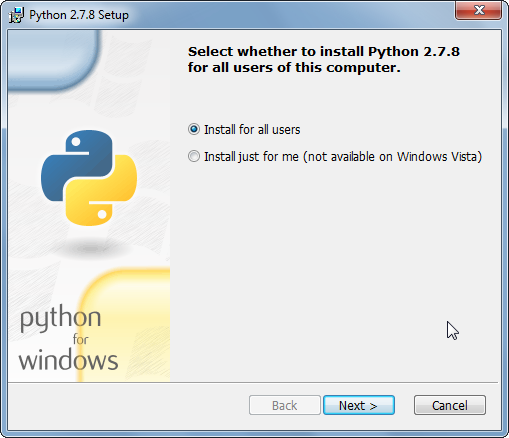
\includegraphics[width=0.45\textwidth]{python/install/037.png}
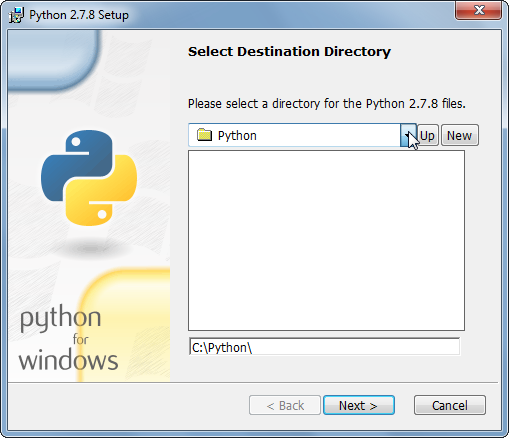
\includegraphics[width=0.45\textwidth]{python/install/038.png}
\bigskip

\menu{Customize > Python > Add python.exe to PATH > Next > Finish}

\nopagebreak
\bigskip
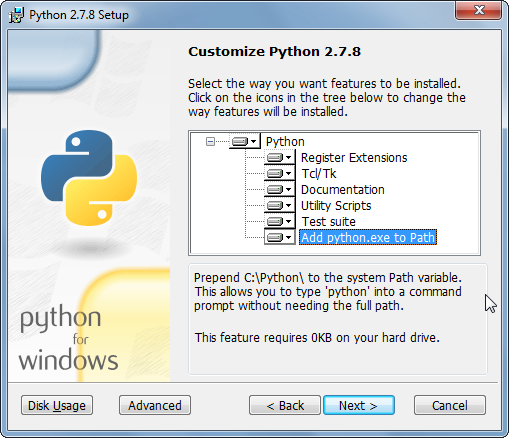
\includegraphics[width=0.45\textwidth]{python/install/039.png}
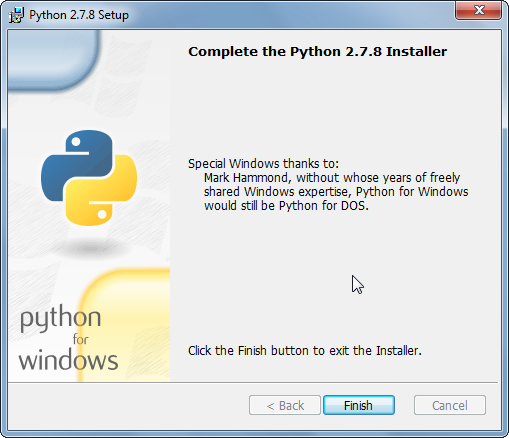
\includegraphics[width=0.45\textwidth]{python/install/045.png}
\bigskip

\section{Запуск}

Из командной строки: \menu{\winr cmd > python}

\bigskip
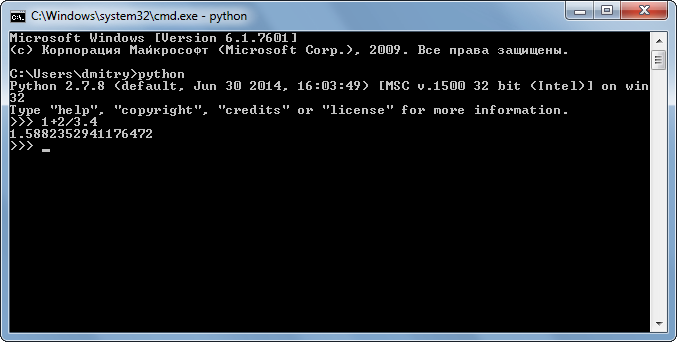
\includegraphics[width=0.9\textwidth]{python/install/046.png}
\bigskip

Простейшая среда IDLE\note{на GUI-библиотеке Tkinter, идущей в комплекте}:
\bigskip

\menu{\winstart > Программы > Python 2.7 > IDLE (Python GUI)}

\menu{Панель задач > IDLE > \rms > Закрепить в панели задач > \lms }

\bigskip
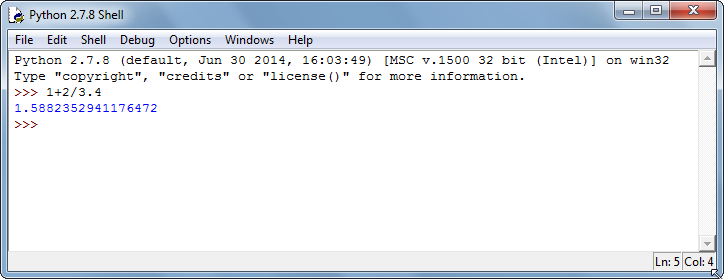
\includegraphics[width=0.9\textwidth]{python/install/047.png}
\bigskip

\dblms\ по файлу скрипта:
\bigskip

\menu{\winr > notepad \file{/tmp/py.py}}

\lst{/tmp/py.py}{}{python/install/py.py}

\menu{\winr > /tmp/py.py}

\bigskip
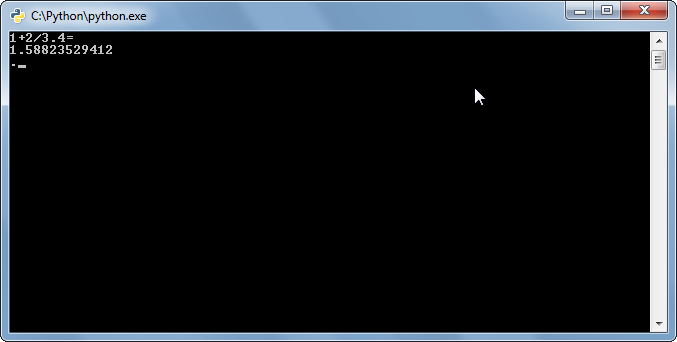
\includegraphics[width=0.9\textwidth]{python/install/048.png}
\bigskip

Открытием файла скрипта в IDLE:
\bigskip

\menu{\winr > \file{/tmp/}}

\menu{\file{py.py} > \rms > Edit with IDLE}

\menu{меню > Run > Run Module \keys{F5}}

\bigskip
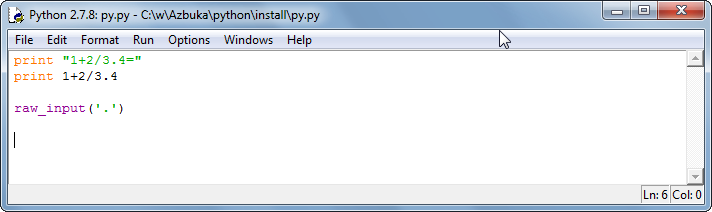
\includegraphics[width=0.9\textwidth]{python/install/049.png}

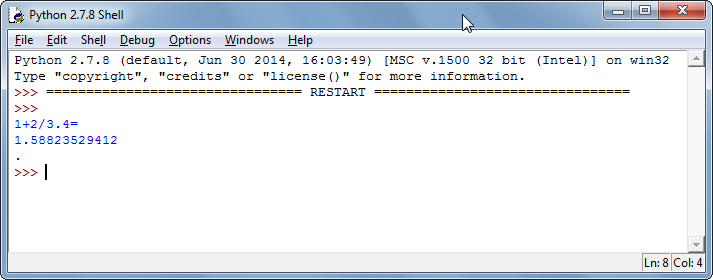
\includegraphics[width=0.9\textwidth]{python/install/050.png}
\bigskip

\section{Дополнительные материалы}

\cite{pyotkidach} Г. Россум, Ф.Л.Дж. Дрейк, Д.С. Откидач,
\href{http://rus-linux.net/MyLDP/BOOKS/python.pdf}{Язык программирования Python}

\cite{pythink} Аллен Дауни
\href{https://drive.google.com/file/d/0B0u4WeMjO894Q2hWV1QwOFFQOVk/view?usp=sharing}{Думать
на языке \py: Думать как компьютерный специалист}

